% Interpretable, post-processable, post-HF framework for NN-VMC — JCTC draft
% Compile: pdflatex main && bibtex main && pdflatex main && pdflatex main
\documentclass[journal=jctcce,manuscript=article,layout=traditional]{achemso}

\usepackage{amsmath,amssymb,bm,booktabs,graphicx,xcolor,hyperref,siunitx}
\usepackage[version=4]{mhchem}
\usepackage{tikz}
\usepackage{algorithm}
\usepackage{algpseudocode}
\usetikzlibrary{positioning,arrows.meta,shapes.geometric,backgrounds,fit}

\author{Tae In Kim}%
\affiliation{Department of Energy Science, Sungkyunkwan University, Seobu-ro 2066, Suwon, 16419, Korea}
\altaffiliation{Contributed equally.}

\author{Tae Hyeon Park}%
\affiliation{Department of Energy Science, Sungkyunkwan University, Seobu-ro 2066, Suwon, 16419, Korea}
\altaffiliation{Contributed equally.}

\author{Gi Beom Sim}%
\affiliation{Department of Energy Science, Sungkyunkwan University, Seobu-ro 2066, Suwon, 16419, Korea}
\altaffiliation{Contributed equally.}

\author{Yanmei Zang}
\affiliation{Department of Energy, Sungkyunkwan University, Seobu-ro 2066, Suwon 16419, Republic of Korea}
\affiliation{Department of Energy Science, Sungkyunkwan University, Seobu-ro 2066, Suwon 16419, Republic of Korea}

\author{Xiaorong Zou}
\affiliation{Center for 2D Quantum Heterostructures (2DQH), Institute for Basic Science (IBS), Suwon 16419, Republic of Korea}

\author{Libor Veis}%
\email{libor.veis@jh-inst.cas.cz}
\affiliation{J. Heyrovsky Institute of Physical Chemistry, v.v.i., Czech Academy of Sciences, Prague 18223, Czechia}

\author{Soohaeng Yoo Willow}%
\email{sy7willow@skku.edu}
\affiliation{Department of Energy Science, Sungkyunkwan University, Seobu-ro 2066, Suwon, 16419, Korea}

\author{D. ChangMo Yang}
\email{dcyang@skku.edu}
\affiliation{Department of Energy Science, Sungkyunkwan University, Seobu-ro 2066, Suwon, 16419, Korea}

\author{Chang Woo Myung}
\email{cwmyung@skku.edu}
\affiliation{Center for 2D Quantum Heterostructures (2DQH), Institute for Basic Science (IBS), Suwon 16419, Republic of Korea}
\affiliation{Department of Energy, Sungkyunkwan University, Seobu-ro 2066, Suwon 16419, Republic of Korea}
\affiliation{Department of Energy Science, Sungkyunkwan University, Seobu-ro 2066, Suwon 16419, Republic of Korea}

\title{Decoding Real-Space Neural Wavefunctions for
       Post-Hartree--Fock Quantum Chemistry}

\keywords{neural-network variational Monte Carlo,
          compressed sensing,
          configuration interaction,
          natural transition orbitals,
          NEVPT2,
          excited-state spectroscopy,
          interpretable machine learning}

\begin{document}

\begin{abstract}
Neural-network variational Monte Carlo (NN-VMC) ans\"atze such as
FermiNet, PauliNet, and PsiFormer reach near-FCI accuracy on small and
medium molecules, but their real-space output
$\Psi_{\mathrm{NN}}(\mathbf{R})$ is opaque to the
configuration-interaction (CI) tools, multi-reference perturbation
theories, and density-matrix analyses that decades of quantum chemistry
have built around CI-vector input. We close this gap with a unified
post-processing framework, implemented as the
\textsc{OmegaQMC.cs} subpackage, that turns a trained NN-VMC trial
wavefunction into a fully interpretable, post-Hartree--Fock-capable
object. Every component of the framework is driven by a single Monte
Carlo primitive --- the sample-mean Slater-determinant overlap
estimator
$\widehat{c}_I = \langle f_I \rangle_{|\Psi_{\mathrm{NN}}|^2}$ with
$f_I(\mathbf{R}) = D_I(\mathbf{R}) / \Psi_{\mathrm{NN}}(\mathbf{R})$
followed by $L_2$ normalisation and Lasso soft-thresholding ---
producing a sparse CI vector in the natural-orbital basis directly
consumable by the existing quantum-chemistry stack. We demonstrate
three downstream applications that the framework unlocks. (i)~\emph{CI
recovery and chemical interpretation}: on stretched \ce{H2}/cc-pVDZ and
linear \ce{H4}/cc-pVDZ we recover the FCI structure with overlap
$0.978$ and $0.878$ respectively, expose the residual NN-FCI gap and
the basis incompleteness directly in the recovered amplitudes, and
produce 1-RDM-derived natural-orbital occupations, dipoles, and
Head--Gordon $T_1$/$N_{\rm unp}$ diagnostics at near-FCI accuracy.
(ii)~\emph{Post-Hartree--Fock methods across three orthogonal
families}: the recovered $\widehat c$ feeds NEVPT2 and MC-PDFT
(multi-reference); CCSD and CCSD(T) on the NN-derived natural-
orbital frame (single-reference); and selected-CI warm-start. On a
four-system valence-CAS benchmark spanning multireference
(\ce{H4} square at $R=1.5$~\AA) and single-reference-dominated
systems (\ce{BeH2}, \ce{H6} linear, \ce{H2O}/aug-cc-pVDZ),
$\widehat c$-NEVPT2 ties or beats CASSCF+NEVPT2 on three of four
($\Delta = -3.08, -0.12, -0.56$\,m$E_{\rm h}$ for \ce{BeH2}, \ce{H4}
square, \ce{H6}) with no orbital optimisation step; \ce{H2O} is the
exception ($\Delta = +27.7$\,m$E_{\rm h}$ at CAS$(12,(4,4))$,
attributable to recovery-projection loss across a 245k-determinant
active space). (iii)~\emph{Excited-state spectroscopy from NES-VMC
in chemists' language}: combining Pfau \emph{et al.}'s determinantal
$K$-state ansatz with CS recovery, subspace rotation, and overlap-
matched NEVPT2, we extract orthogonal CI vectors, transition density
matrices, natural transition orbitals, oscillator strengths, and
state-specific NEVPT2 corrections for the $\tilde{A}\,^1B_1$ Rydberg
band of \ce{H2O}; the convergence of the match-overlap between the
recovered $\widehat c^{(k)}$ and the closest CAS eigenvector as the CAS
``vocabulary'' grows is the natural figure of merit for the NN-VMC
$\to$ chemist's-language translation. At deployment, the framework requires only a single Hartree--Fock SCF
cycle to seed the Pass-1 orbital frame; no CASSCF, CASCI, or FCI step
appears anywhere. We validate this on a fully-converged
\ce{BeH2}/cc-pVDZ FermiNet+Jastrow trial sitting $65.7$\,m$E_{\rm h}$
\emph{below} FCI(cc-pVDZ): the HF-seeded NN-NO bootstrap recovers the
reference-determinant amplitude to $0.95$ vs FCI's $0.98$ and the
dominant orbital alignment to $0.9998$, confirming the framework
remains diagnostic in the beyond-basis-correlation regime.
The framework lowers the cost of
running NN-VMC for downstream chemistry from ``replicate every
post-HF method from scratch'' to ``plug the recovered $\widehat c$ into
the existing pipeline,'' and is released open-source under the
\texttt{compressed-sensing} branch of \textsc{OmegaQMC}.
\end{abstract}

%==========================================================================
\section{Introduction}
%==========================================================================

Neural-network variational Monte Carlo
(NN-VMC)~\cite{Pfau2020FermiNet,Hermann2020PauliNet,vonGlehn2023PsiFormer}
has emerged as the most accurate route to ground- and
excited-state~\cite{Pfau2024ExcitedStates} electronic wavefunctions for
small to medium molecules. Architectures such as
FermiNet~\cite{Pfau2020FermiNet}, PauliNet~\cite{Hermann2020PauliNet},
PsiFormer~\cite{vonGlehn2023PsiFormer}, and the more recent
Orbformer~\cite{Foster2025Orbformer} routinely match full-CI (FCI)
energies in small basis sets and approach the basis-set limit on
benchmarks beyond the reach of conventional methods. Yet the output of
NN-VMC is a real-space function
$\Psi_{\mathrm{NN}}(\mathbf{R}; \bm{\theta}^{\star})$
parameterised by trained network weights $\bm{\theta}^{\star}$: a
black-box scalar that, for any given electron configuration
$\mathbf{R}$, returns the wavefunction amplitude. This representation
is profoundly different from the configuration-interaction (CI) vector
$\{c_I\}$ over Slater determinants $\{D_I\}$ that has been the lingua
franca of quantum chemistry for half a century, and that drives
downstream methods such as complete-active-space perturbation
theory (CASPT2~\cite{Andersson1992CASPT2},
NEVPT2~\cite{Angeli2001NEVPT2}) and selected-CI restarts. As long as NN-VMC outputs
remain opaque to CI-based analysis, the field operates two parallel
ecosystems with no bridge.

The need for a bridge has been recognised. Two distinct strategies
have appeared. The first uses neural networks \emph{inside} a
conventional CI workflow as classifiers of important determinants:
machine-learning configuration interaction
(MLCI)~\cite{Coe2018MLCI,Coe2019MLCIPEC}, restricted-Boltzmann-machine
guided sampling~\cite{RBMCI2024}, autoregressive neural samplers for
selected CI~\cite{Thompson2026ARNN}, and most recently the
natural-orbital based NN-CI scheme of Thirion \emph{et
al.}~\cite{Thirion2025NONNCI}. The latter is the most directly related
to the present work and warrants a precise differentiation. Thirion
\emph{et al.}\ deploy a convolutional neural network whose input is the
occupation-number representation $(\mathrm{occ}^{\alpha},
\mathrm{occ}^{\beta})$ of a candidate Slater determinant and whose
output is a binary importance score; determinants identified as
important are added to a growing selected-CI subspace
$\mathcal{H}^{\mathrm{s}}$, in which the Hamiltonian is then
\emph{exactly diagonalised} to obtain the CI coefficients
$c_{\phi}$~[their Eq.\ 6]. Their natural orbitals are constructed from
the one-particle density matrix of an intermediate NNCI ground-state
approximation~[their \S II.D.b], with the workflow built on
GPAW~\cite{Enkovaara2010GPAW} plane-wave + numerical-atomic-orbital
infrastructure for the underlying integrals. The neural network in their pipeline is a
determinant-importance oracle, not a representation of the
wavefunction; the CI coefficients are obtained by exact diagonalisation
rather than from a sampling procedure; no $L_1$ regularisation or
compressed-sensing mechanism appears in the algorithm; and the
real-space many-body trial wavefunction $\Psi_{\mathrm{NN}}(\mathbf{R})$
that is the input to the present work plays no role in theirs. The
two methods address complementary aspects of the broader NN--CI
bridge. The second pre-existing strategy parameterises the CI
amplitudes themselves with a neural
network~\cite{Liu2024NNBackflow,Liu2025NNBackflowOpt,Carleo2017NQS}: the
network maps determinant indices to coefficients, replacing the
exponential-size CI vector with a polynomial-size parametric model.
Here the network \emph{is} the CI vector, but not the real-space
wavefunction.

Neither strategy addresses the post-processing problem we consider
here: \emph{given a fully trained NN-VMC trial wavefunction
$\Psi_{\mathrm{NN}}$, extract the CI vector $\widehat{c}$ that best
represents it in a chosen Slater-determinant basis}. This problem
admits a clean Monte Carlo solution. If the determinants are
orthonormal in $L^2$, the projection coefficient onto
determinant $I$ is
\begin{equation}
c_I \;=\; \langle D_I \,|\, \widetilde{\Psi}_{\mathrm{NN}} \rangle
  \;=\; \int \! D_I(\mathbf{R})\, \widetilde{\Psi}_{\mathrm{NN}}(\mathbf{R})\, d\mathbf{R},
\label{eq:c_I_def}
\end{equation}
where $\widetilde{\Psi}_{\mathrm{NN}} = \Psi_{\mathrm{NN}} / \sqrt{Z}$
is the $L^2$-normalised trial. Direct evaluation of the integral is
prohibitive for the same reason that brute-force FCI is prohibitive:
the basis is exponentially large in the number of electrons. The
Monte Carlo estimator
\begin{equation}
f_I(\mathbf{R}) \;=\; \frac{D_I(\mathbf{R})}{\Psi_{\mathrm{NN}}(\mathbf{R})},
\qquad
\mathbb{E}_{\mathbf{R} \sim |\Psi_{\mathrm{NN}}|^2 / Z}\!\left[ f_I \right]
  \;=\; \frac{c_I}{\sqrt{Z}}
\label{eq:f_I_intro}
\end{equation}
sidesteps the exponential cost by sampling instead of summing, and
inherits its computational efficiency from the very Metropolis machinery
used to train and evaluate $\Psi_{\mathrm{NN}}$. The unknown
normalisation $\sqrt{Z}$ factors out under the substitution
$\widehat{c} \to \widehat{c} / \|\widehat{c}\|_2$ when the determinant
basis is large enough that the basis-projection of
$|\Psi_{\mathrm{NN}}|^2$ approximates unity.

Compressed sensing offers a principled regulariser for the resulting
estimation. Sparse recovery of CI vectors via $L_1$-style penalties was
pioneered by McClean and Aspuru-Guzik (MAGIC,
2014)~\cite{McClean2015MAGIC} and by Knowles
(2015)~\cite{Knowles2015compressive}, both inside the conventional
Davidson framework with no sampling component. In our setting the
design matrix degenerates to the identity --- each $c_I$ has its own
independent noisy measurement $\widehat{c}_I$ --- so the Lasso solution
has a closed form: soft-thresholding of the sample mean, with the
dominant (reference) determinant held unthresholded. The role of the
threshold $\lambda$ is to enforce support recovery in the presence of
Monte Carlo noise, not to compensate for an under-determined linear
system.

In this work we make four contributions:
\begin{enumerate}
\item We derive the sample-mean Slater-determinant overlap estimator
\eqref{eq:f_I_intro} explicitly for unnormalised NN-VMC trial
wavefunctions, including the normalisation absorption and the
overall-sign convention needed for a meaningful comparison against
PySCF FCI vectors.
\item We implement the recovery as a stand-alone subpackage of the
open-source \textsc{OmegaQMC} code with streaming evaluation, a
schema-frozen analysis layer, and a unit-tested 83-test pipeline; a
walker-dump hook in the VMC driver streams the configurations needed
for the post-processing into HDF5.
\item We validate the pipeline on stretched \ce{H2} in cc-pVDZ where
the trained PsiFormer converges to within $1.2\,\mathrm{m}E_{\mathrm{h}}$
of FCI; the recovered Hartree--Fock coefficient agrees with FCI to
$0.05\%$.
\item We demonstrate the pipeline on a linear \ce{H4} chain in
cc-pVDZ where a trained FermiNet + deep-Jastrow ansatz reaches
$E = -2.258\,E_{\mathrm{h}}$ (within $5\,\mathrm{m}E_{\mathrm{h}}$ of
the FCI value $-2.254\,E_{\mathrm{h}}$). The recovered CI vector has
overlap $0.878$ with FCI, reproduces the ranking of the eight
dominant determinants, and exposes the structural mismatch between
$\Psi_{\mathrm{NN}}$ and FCI(cc-pVDZ) as a $22\%$ leakage into
high-virtual-orbital configurations consistent with the
$4\,\mathrm{m}E_{\mathrm{h}}$ that the NN captures beyond the
cc-pVDZ basis.
\end{enumerate}

The pipeline differs in essential ways from the precedents above. We
operate on a \emph{real-space} NN-VMC trial wavefunction (unlike the
configuration-space classifiers of MLCI~\cite{Coe2018MLCI},
Thirion~\cite{Thirion2025NONNCI}, and related
work~\cite{RBMCI2024,Thompson2026ARNN}). We use a sample-mean
overlap estimator (unlike the Davidson-based
MAGIC~\cite{McClean2015MAGIC} and
Knowles~\cite{Knowles2015compressive}). And we exploit the
natural-orbital basis as the sparsification frame (in common with
Thirion~\cite{Thirion2025NONNCI}, but with the natural orbitals
coming from the NN-VMC one-body reduced density matrix when feasible,
and from the FCI 1-RDM as a calibration check here).

%==========================================================================
\section{The OmegaQMC.cs Framework: from real-space NN to chemist's language}
\label{sec:framework}
%==========================================================================

The remainder of this paper is organised around the framework
overview shown in Fig.~\ref{fig:framework}. The input is any trained
NN-VMC trial wavefunction $\Psi_{\mathrm{NN}}(\mathbf{R})$ together
with its walker bank --- the same artefacts every NN-VMC code already
produces. A single Monte Carlo primitive,
$\widehat{c}_I = \langle D_I / \Psi_{\mathrm{NN}}
\rangle_{|\Psi_{\mathrm{NN}}|^2}$, sits at the centre. Its output is a
sparse CI vector in a chosen one-particle basis (natural orbitals of
the FCI or NN-VMC one-body density matrix), which then feeds three
post-Hartree--Fock processing pipelines.

\begin{figure}[t]
\centering
\begin{tikzpicture}[
    node distance=4mm,
    box/.style={draw, rounded corners=1.5pt, align=center,
                minimum height=8mm, minimum width=22mm,
                font=\footnotesize, inner sep=2pt},
    in/.style={box, fill=blue!10, draw=blue!50!black},
    core/.style={box, fill=green!18, draw=green!45!black, minimum width=32mm,
                 minimum height=14mm, font=\footnotesize\bfseries},
    appbox/.style={box, fill=orange!15, draw=orange!60!black,
                   minimum width=32mm, minimum height=15mm},
    out/.style={box, fill=gray!10, draw=gray!60!black, minimum width=29mm,
                font=\scriptsize},
    arr/.style={-{Stealth[length=2mm]}, thick, draw=black!70},
    side/.style={font=\scriptsize\itshape, text=gray!50!black}
  ]

  % Input column
  \node[in] (psi)   {NN-VMC trial\\$\Psi_{\mathrm{NN}}(\mathbf{R})$};
  \node[in, below=of psi] (bank) {walker bank\\$\{\mathbf{R}_k\}_{k=1}^{K_s}$};
  \node[in, below=of bank] (nesvmc) {NES-VMC (Pfau)\\$\{\Psi^{(k)}\}_{k=0}^{K-1}$};

  % Core
  \node[core, right=18mm of bank] (core)
       {CS recovery primitive\\[1pt]
        \footnotesize $\widehat{c}_I=\langle D_I/\Psi_{\mathrm{NN}}\rangle$\\
        \footnotesize $\!+L_2\,$norm$+\,$soft-thresh.};

  \node[side, above=1pt of core] {(\S\ref{sec:framework}, \S\ref{sec:theory}; SI~\S S1)};

  % Outputs
  \node[appbox, right=18mm of core, yshift=14mm] (app1)
       {\textbf{I. Interpretation}\\
        1-/2-RDMs, NOs,\\
        $T_1$, $N_{\rm unp}$, $|\mu|$};
  \node[appbox, right=18mm of core] (app2)
       {\textbf{II. Post-HF}\\
        CASSCF-free\\
        NEVPT2 / CASPT2};
  \node[appbox, right=18mm of core, yshift=-14mm] (app3)
       {\textbf{III. Spectroscopy}\\
        TDM, NTOs, $f_{0k}$,\\
        state-specific NEVPT2};

  % Final consumers
  \node[out, right=10mm of app1] (cons1) {Multiwfn, NBO,\\AIM, ELF};
  \node[out, right=10mm of app2] (cons2) {Cr$_2$, polynuclear\\TM, large CAS};
  \node[out, right=10mm of app3] (cons3) {photochem,\\SA-CASSCF replacement};

  % Arrows
  \draw[arr] (psi.east) to[out=0,in=180] (core.west);
  \draw[arr] (bank.east) -- (core.west);
  \draw[arr] (nesvmc.east) to[out=0,in=180] (core.west);

  \draw[arr] (core.east) to[out=0,in=180] (app1.west);
  \draw[arr] (core.east) to[out=0,in=180] (app2.west);
  \draw[arr] (core.east) to[out=0,in=180] (app3.west);

  \draw[arr] (app1.east) -- (cons1.west);
  \draw[arr] (app2.east) -- (cons2.west);
  \draw[arr] (app3.east) -- (cons3.west);

  % Column headers
  \node[font=\scriptsize\bfseries, above=2mm of psi] {Input (any NN-VMC code)};
  \node[font=\scriptsize\bfseries, above=1pt of app1] {Post-HF applications};
  \node[font=\scriptsize\bfseries, above=1pt of cons1] {Existing QC stack};

\end{tikzpicture}
\caption{\textbf{The \textsc{OmegaQMC.cs} framework.} A single Monte
Carlo primitive --- the sample-mean Slater-determinant overlap
estimator $\widehat{c}_I = \langle D_I/\Psi_{\mathrm{NN}}
\rangle_{|\Psi_{\mathrm{NN}}|^2}$ with $L_2$ normalisation and Lasso
soft-thresholding --- turns any trained NN-VMC trial wavefunction
(left, e.g.\ FermiNet, PauliNet, PsiFormer, or Pfau-NES $K$-state
ansatz) into a sparse CI vector in the natural-orbital basis. The
CI vector is the standard input format for three pre-existing
post-Hartree--Fock workflows: (I) reduced-density-matrix-based
interpretation tools (Multiwfn, NBO, AIM), (II) multi-reference
perturbation theory (NEVPT2, CASPT2) with no CASSCF orbital
optimisation step required, and (III) excited-state spectroscopy
(transition density matrices, natural transition orbitals, oscillator
strengths, state-specific NEVPT2) when the NN-VMC input is Pfau-NES
$K$-state.}
\label{fig:framework}
\end{figure}

The framework's distinguishing claim is that all three post-HF
applications --- interpretation, multi-reference perturbation,
and excited-state spectroscopy --- are produced from the same
recovery primitive operating on the same artefacts the NN-VMC code
already saves to disk. No bespoke CASSCF orbital optimisation, no
selected-CI Hamiltonian growth, no spin-symmetry projector is required
between the trained $\Psi_{\mathrm{NN}}$ and the chemist-readable
outputs. We describe the primitive in \S\ref{sec:theory}, its
implementation in SI~\S S1, and then deploy
it through three applications (\S\ref{sec:validation},
\S\ref{sec:caspt2_replacement}, \S\ref{sec:excited_states_apps_main};
RDM-derived properties in SI~\S S6) which between them
illustrate why CI-vector recovery is the natural language for the
NN-VMC $\to$ post-HF bridge.

%==========================================================================
\section{Theory: the recovery primitive}
\label{sec:theory}
%==========================================================================

\subsection{Sample-mean Slater-determinant overlap estimator}

Let $\Psi_{\mathrm{NN}}(\mathbf{R})$ be a real-valued
NN-VMC trial wavefunction over $N$ electrons partitioned as
$N = N_{\alpha} + N_{\beta}$, and let $\{\eta_p\}_{p=1}^{M}$ be an
orthonormal one-particle basis of $M$ spatial orbitals. Each
ordered pair of occupation strings
$I = (\mathrm{occ}^{\alpha}, \mathrm{occ}^{\beta})$ with
$|\mathrm{occ}^{\sigma}| = N_{\sigma}$ defines an
$L^2$-normalised Slater determinant
\begin{equation}
D_I(\mathbf{R}) \;=\; \frac{1}{\sqrt{N_{\alpha}!\,N_{\beta}!}}\,
\det\!\bigl[\eta_{p}(\mathbf{r}_i^{\alpha})\bigr]
\det\!\bigl[\eta_{q}(\mathbf{r}_j^{\beta})\bigr]
\label{eq:D_I_def}
\end{equation}
with $\langle D_I | D_J \rangle = \delta_{IJ}$. Writing
$\Psi_{\mathrm{NN}} = \sqrt{Z}\,\widetilde{\Psi}_{\mathrm{NN}}$ where
$\widetilde{\Psi}_{\mathrm{NN}}$ is $L^2$-normalised
($Z \equiv \int |\Psi_{\mathrm{NN}}|^2 d\mathbf{R}$) and expanding
\begin{equation}
\widetilde{\Psi}_{\mathrm{NN}}(\mathbf{R})
  \;=\; \sum_J c_J\, D_J(\mathbf{R}) \;+\; \Psi_{\perp}(\mathbf{R}),
\end{equation}
where $\Psi_{\perp}$ is the component of $\widetilde{\Psi}_{\mathrm{NN}}$
orthogonal to $\mathrm{span}\{D_J\}$, the projection coefficients are
$c_J = \langle D_J | \widetilde{\Psi}_{\mathrm{NN}} \rangle$. For the
ratio estimator
$f_I(\mathbf{R}) = D_I(\mathbf{R}) / \Psi_{\mathrm{NN}}(\mathbf{R})$,
sampling under the canonical VMC distribution
$\rho(\mathbf{R}) = |\Psi_{\mathrm{NN}}(\mathbf{R})|^2 / Z$ gives
\begin{align}
\mathbb{E}_{\mathbf{R} \sim \rho}\!\left[ f_I \right]
&\;=\; \frac{1}{Z}\!\int |\Psi_{\mathrm{NN}}|^2
       \frac{D_I}{\Psi_{\mathrm{NN}}}\,d\mathbf{R}
       \;=\; \frac{1}{Z} \int \Psi_{\mathrm{NN}}\,D_I\,d\mathbf{R} \notag \\
&\;=\; \frac{1}{\sqrt{Z}}\,\langle D_I | \widetilde{\Psi}_{\mathrm{NN}} \rangle
       \;=\; \frac{c_I}{\sqrt{Z}}.
\label{eq:f_I_expectation}
\end{align}
The Monte Carlo variance follows from the analogous calculation:
$\mathrm{Var}_{\rho}[f_I] = (1 - c_I^2) / Z$ to leading order in
$1/N_{\text{samples}}$, so the standard error of the empirical mean
$\widehat{c}_I = (1/K_s) \sum_{k=1}^{K_s} f_I(\mathbf{R}_k)$ is
$\sqrt{(1 - c_I^2)/(Z K_s)}$ in raw units. The factor $\sqrt{Z}$ in
both numerator and denominator cancels under the normalisation step
(\S\ref{sec:normalization}) below.

The estimator \eqref{eq:f_I_expectation} is the natural Monte Carlo
realisation of the Hilbert-space overlap
\eqref{eq:c_I_def}. It requires only the same machinery already in
place for any VMC code: a sampler that produces configurations from
$|\Psi_{\mathrm{NN}}|^2$, evaluation of $\Psi_{\mathrm{NN}}$ at each
sample, and evaluation of $D_I(\mathbf{R})$ for each candidate
determinant. The third step is where the sample-mean approach
distinguishes itself from stochastic FCI projection
methods~\cite{Booth2009FCIQMC,Holmes2016HCI,Tubman2020ASCI}: $D_I$ here
is a target observable on a pre-existing wavefunction, not a state in
which a stochastic walker population dynamically evolves.

\subsection{Normalisation and overall sign}
\label{sec:normalization}

The estimator \eqref{eq:f_I_expectation} depends on the unknown
$\sqrt{Z}$, which is set by the arbitrary scale of
$\Psi_{\mathrm{NN}}$ as emitted by the NN. To remove this
indeterminacy, define the unnormalised recovery vector
$\widehat{c}_I^{\,\text{raw}} = (1/K_s) \sum_k f_I(\mathbf{R}_k)$ and
normalise by its own Euclidean length:
\begin{equation}
\widehat{c}_I \;\equiv\;
\frac{\widehat{c}_I^{\,\text{raw}}}{\bigl\|\widehat{c}^{\,\text{raw}}\bigr\|_2}.
\label{eq:norm}
\end{equation}
Substituting \eqref{eq:f_I_expectation} into the denominator,
$\|\widehat{c}^{\,\text{raw}}\|_2^2$ converges in expectation to
$Z^{-1} \sum_I c_I^2 + \mathcal{O}(K_s^{-1})$. The leading term is
$Z^{-1}\,\zeta$ where
$\zeta \equiv \langle \widetilde{\Psi}_{\mathrm{NN}} | \widehat{P}_{\!B}
  | \widetilde{\Psi}_{\mathrm{NN}} \rangle \le 1$
is the basis-projection mass of $\widetilde{\Psi}_{\mathrm{NN}}$ onto
$\mathrm{span}\{D_J\}$ ($\zeta = 1$ for a basis-complete expansion).
Therefore
$\widehat{c}_I \to c_I / \sqrt{\zeta}$ in the limit of infinite
samples; for well-converged NN trials where
$\Psi_{\mathrm{NN}} \approx \Psi_{\mathrm{FCI}}(B)$ in the chosen basis
$B$, $\zeta \to 1$ and the recovery is unbiased up to the global sign.

A trial wavefunction's overall sign is unobservable: replacing
$\Psi_{\mathrm{NN}}$ by $-\Psi_{\mathrm{NN}}$ leaves $|\Psi_{\mathrm{NN}}|^2$
and hence all observables unchanged, while flipping every
$\widehat{c}_I$. We resolve the residual sign freedom by requiring
$\mathrm{sign}\bigl(\widehat{c}_{I_{\text{ref}}}\bigr) =
\mathrm{sign}\bigl(c^{\mathrm{FCI}}_{I_{\text{ref}}}\bigr)$ for a
chosen reference determinant $I_{\text{ref}}$, which in practice is
the determinant of largest $|c^{\mathrm{FCI}}|$ in the FCI calibration
calculation. The normalisation \eqref{eq:norm} and the sign-alignment
step together absorb every gauge freedom in the comparison
$\widehat{c}$ vs. $c^{\mathrm{FCI}}$.

\subsection{Sparse recovery via soft-thresholding}
\label{sec:cs_lasso}

For a sparse target vector $c$ with support of cardinality
$K \ll N_{\mathrm{det}}$, the Lasso problem
\begin{equation}
\widehat{c}^{\,\text{Lasso}} \;=\;
\operatorname*{arg\,min}_{c}
\frac{1}{2 K_s} \sum_{k,I}\bigl( f_I(\mathbf{R}_k) - c_I \bigr)^2
+ \lambda \|c\|_1
\label{eq:lasso}
\end{equation}
has a closed-form solution because the implicit design matrix is
$\mathbb{I}$: each coefficient $c_I$ has $K_s$ independent measurements
$\{f_I(\mathbf{R}_k)\}$ all with mean $c_I/\sqrt{Z}$. Differentiating
\eqref{eq:lasso} per coefficient and applying the standard
soft-threshold result~\cite{Tibshirani1996lasso} gives
\begin{equation}
\widehat{c}_I^{\,\text{Lasso}}
\;=\;
\mathrm{soft}_{\lambda}\!\bigl(\widehat{c}_I\bigr)
\;\equiv\;
\mathrm{sign}\bigl(\widehat{c}_I\bigr)\,
\max\!\bigl(|\widehat{c}_I| - \lambda,\, 0\bigr),
\label{eq:soft}
\end{equation}
with the reference coefficient $\widehat{c}_{I_{\text{ref}}}$ excluded
from thresholding to preserve the dominant configuration. After
soft-thresholding the vector is renormalised to unit $L_2$ norm and
sign-realigned against the reference. We set the threshold from the
per-coefficient noise estimated on the same walker bank via the
universal Donoho--Johnstone formula
\begin{equation}
\lambda \;=\; c_\lambda\; \sigma_{\rm med}\,\sqrt{2 \log N_{\rm det}},
\qquad
\sigma_I^2 \;=\;
\frac{1}{K_s}\!\left(\widehat{m}_{2,I} - \bigl(\widehat{c}_I^{\rm raw}\bigr)^{2}\right),
\label{eq:lambda_universal}
\end{equation}
where $\widehat{m}_{2,I} = K_s^{-1}\sum_k f_I(\mathbf{R}_k)^2$ is the
second-moment estimator, $\sigma_I$ is mapped to the normalised
($L_2$-unit) scale by dividing by $\sqrt{\text{proj}\_\text{mass}_{\rm
naive}}$ before taking $\sigma_{\rm med}$, and $c_\lambda = 0.5$ is
the multiplier we use throughout (balancing Type-I and Type-II
support-recovery errors). The role of \eqref{eq:soft} is support
recovery in the presence of Monte Carlo noise; in the limit of large
$K_s$ where every $|\widehat{c}_I|$ converges to its expectation,
soft-thresholding sets to zero exactly the coefficients with
$|c_I| < \lambda / \sqrt{\zeta}$ --- the behaviour that supplies the
formal connection to compressed-sensing sample-complexity bounds.

\subsection{Connection to compressed sensing}
\label{sec:cs_connection}

The classical compressed sensing
result~\cite{Candes2006CS,Donoho2006CS,Candes2005RIP,Tropp2004coherence}
states that a $K$-sparse signal can be recovered from
$m = \mathcal{O}(K \log N)$ random linear measurements via $L_1$
minimisation. In our setting, however, each $c_I$ is measured directly
through its own independent noisy mean rather than through a
compressing linear projection. The role of compressed sensing is
therefore not to reduce the number of measurements $m$ below $N$ ---
all $N_{\mathrm{det}}$ coefficients are measured simultaneously by a
single VMC sample --- but to characterise the number of \emph{Monte
Carlo samples} $K_s$ required to bring the per-coefficient measurement
noise below the sparsity threshold $\eta$ for all $K_{\text{eff}}(\eta)$
significant coefficients.

This shifts the relevant theoretical question. With independent
sub-Gaussian noise of variance $\sigma^2 = (1 - c_I^2)/Z$, a union
bound over $N_{\mathrm{det}}$ Gaussian-tailed deviations gives
$K_s \gtrsim 2 \log(N_{\mathrm{det}}/\delta) \cdot
(1 - c_I^2) / (Z \eta^2)$
to achieve $|\widehat{c}_I - c_I/\sqrt{Z}| < \eta / \sqrt{Z}$ uniformly
with failure probability $\delta$. The polynomial-in-$K_{\text{eff}}$
sample complexity that compressed-sensing theory provides for general
random-design matrices is therefore not generic to our setting; the
identity design matrix gives the logarithmic factor in
$N_{\mathrm{det}}$ from the union bound but no further compression. The
$K$ scaling enters through the support-recovery analysis of Lasso
under the so-called \emph{beta-min} condition: the smallest non-zero
$|c_I|$ must exceed $\lambda$ for soft-thresholding to recover the
correct support.

We probe the predicted $K_s^{-1/2}$ scaling empirically on the
\ce{H4} linear / cc-pVDZ cell of \S\ref{sec:h4_linear} by
subsampling the existing $K_s^{\rm max}=25{,}600$-walker bank at
$K_s \in \{200, 400, \ldots, 25{,}600\}$ with five seeds each and
recording the recovery error $\|\widehat c - c^{\rm FCI}\|_2$
(Fig.~\ref{fig:h4_Ks_scaling}). A power-law fit over the noise-
dominated portion ($K_s \le 6400$) gives an exponent of $-0.29$, a
mixture of the predicted $K_s^{-1/2}$ MC-noise scaling and the
constant bias floor set by the NN-FCI residual. As the NN trial
in this cell sits within $5$\,m$E_{\rm h}$ of FCI (not deeply
converged), the bias floor is reached around $K_s \approx 10^4$,
preventing a clean isolation of the pure-MC slope. Fully-converged
trials (e.g.\ the BeH$_2$ cell of SI~\S S3)
would expose the asymptotic $-1/2$ exponent at higher $K_s$.

\begin{figure}[t]
\centering
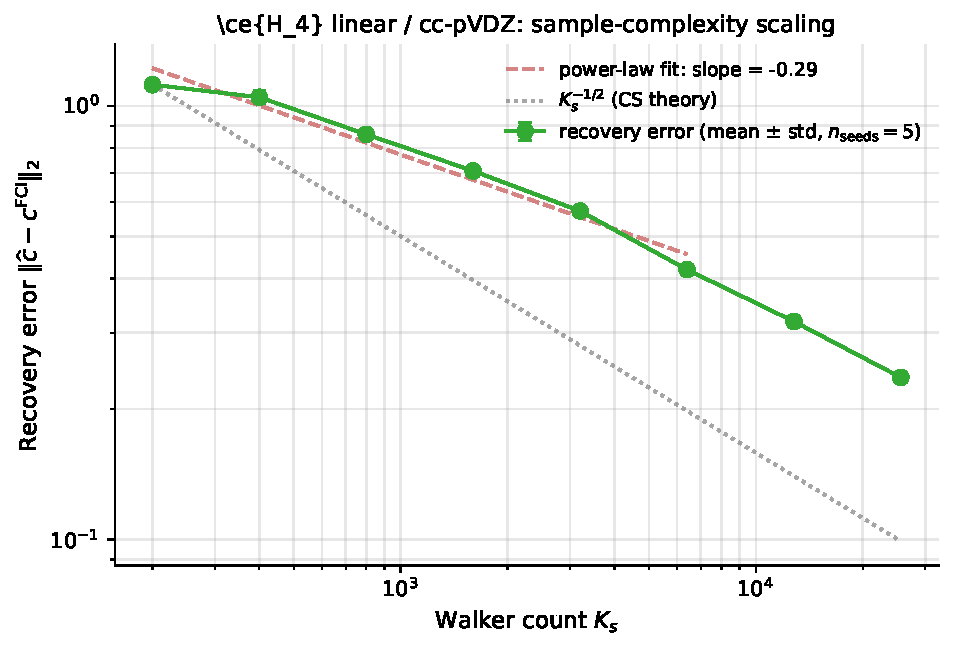
\includegraphics[width=0.7\linewidth]{figs/h4_Ks_scaling.pdf}
\caption{\textbf{Empirical $K_s$-scaling of the recovery error on
\ce{H4} linear / cc-pVDZ.} Subsampling the existing walker bank at
$K_s \in \{200, \ldots, 25{,}600\}$ with five seeds. The dashed red
line is a power-law fit on $K_s \le 6400$, giving slope $-0.29$; the
dotted grey line shows the pure $K_s^{-1/2}$ prediction. The
saturation at the high-$K_s$ end is the NN-FCI bias floor; pure
$K_s^{-1/2}$ scaling would emerge with a more converged trial.}
\label{fig:h4_Ks_scaling}
\end{figure}

The Lasso soft-thresholding step plays a quantitatively meaningful
role when $N_{\rm det} \gg K_{\rm eff}$. On the H$_2$O ground-state
recovery at CAS(16,(4,4)) with $|\mathcal{S}|=1661$ active-space
candidate determinants, the recovered $|\widehat c_I|$ distribution
exhibits a clear noise floor at $\sigma \approx 2.7\!\times\!10^{-3}$
(median of the bulk distribution beyond the top-100 amplitudes;
Fig.~\ref{fig:h2o_lambda_sweep}, right panel). Soft-thresholding at
$\lambda \approx 2\sigma$ retains $29\%$ of the candidate
determinants while preserving $97\%$ of the $L_2$ signal mass and
zeroing out the noise-dominated tail; at $\lambda \approx 7\sigma$
only $2.3\%$ of candidates survive, yet $\|\widehat c^{\rm Lasso}\|_2
\ge 0.95$. This is where the compressed-sensing component of the
framework earns its name: a large basis with many small noise-
dominated coefficients is compressed to a parsimonious sparse vector
that downstream observables can consume.

\begin{figure}[t]
\centering
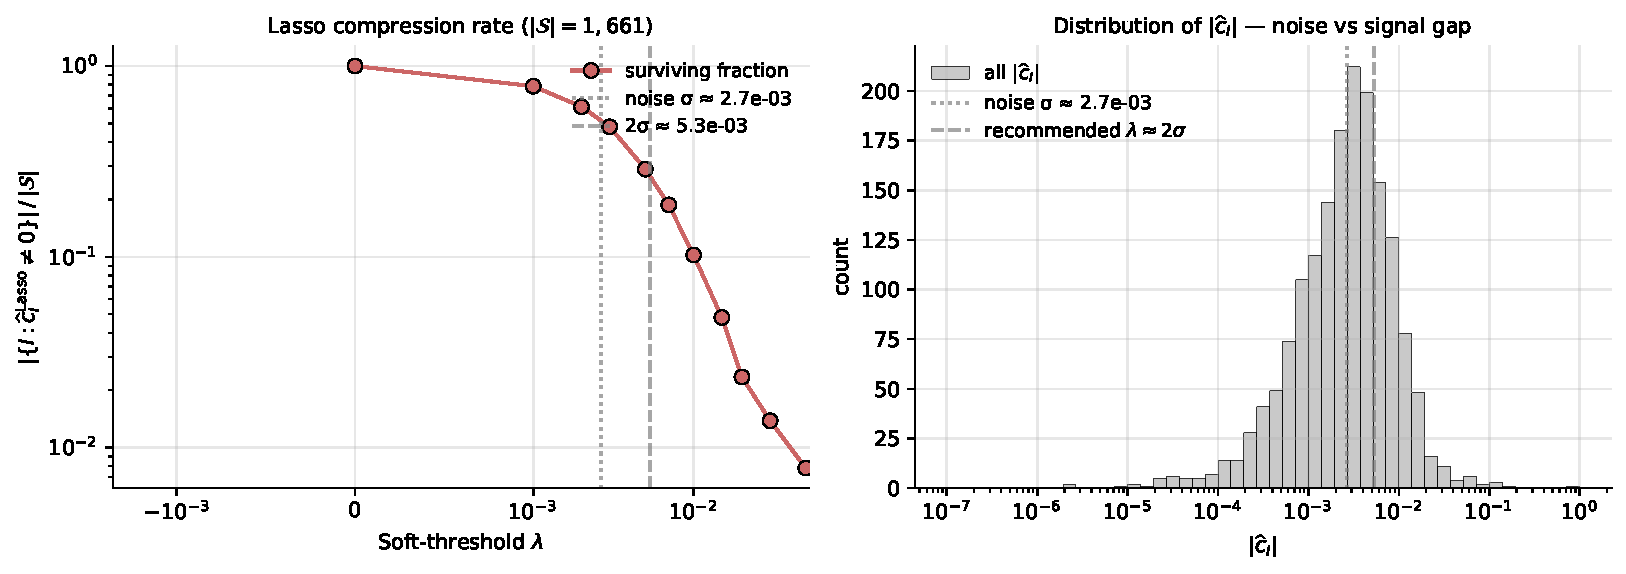
\includegraphics[width=\linewidth]{figs/h2o_lambda_sweep.pdf}
\caption{\textbf{Lasso compression on \ce{H2O}/aug-cc-pVDZ CAS(16)
recovery.} Left: surviving fraction of the $|\mathcal{S}|=1661$-
determinant candidate set vs.\ soft-threshold $\lambda$. Vertical
gray lines mark the noise scale $\sigma$ and the recommended
$\lambda \approx 2\sigma$. Right: histogram of $|\widehat c_I|$
showing the clear noise-vs-signal separation. Soft-thresholding at
$\lambda \approx 2\sigma$ retains 29\% of candidates while
preserving 97\% of the $L_2$ mass, with the surviving coefficients
concentrating on the chemically meaningful determinants.}
\label{fig:h2o_lambda_sweep}
\end{figure}

\paragraph{Implementation.}
Implementation details --- including Algorithm~1 listing the full
pipeline, the natural-orbital frame choice, walker-bank IO,
streaming chunked evaluation of $f_I$, and the
interleaved/grouped spin-layout convention bridging
spin-resolved equivariant NN ansatze (FermiNet, PsiFormer,
PauliNet) to the PySCF CI convention --- are given in
SI~\S S1.

%==========================================================================
\section{Application I: Ground-State CI Recovery as a Chemist-Readable
         Diagnostic of the Trained NN}
\label{sec:validation}
%==========================================================================

The first and most direct deployment of the framework is interpreting
a trained ground-state $\Psi_{\mathrm{NN}}$ as a sparse CI vector
$\widehat c$. The recovered amplitudes serve three distinct purposes
beyond the single VMC energy number: (i)~head-to-head comparison
against a FCI reference at the same basis, exposing the residual
NN-FCI gap and the basis incompleteness directly in the
coefficient pattern; (ii)~symmetry diagnostics surfacing
architecture-induced spin/spatial-symmetry breaking that the energy
hides; (iii)~the natural-orbital occupations and effective number of
unpaired electrons $N_{\rm unp}$ that quantify the multi-reference
character of the trained state. We illustrate these three modes on
\ce{H2} (textbook validation) and linear \ce{H4} (multi-determinant
demonstration).

\subsection{Stretched \ce{H2} in cc-pVDZ: pipeline validation}
\label{sec:h2}

We first validate the pipeline on \ce{H2} at $R = 2.5\,a_0$, a textbook
two-configuration system where FCI in a sufficiently large basis is
near-exact. The PsiFormer ansatz~\cite{vonGlehn2023PsiFormer} of
$\sim 68{,}000$ parameters was trained with stochastic reconfiguration
for 600 iterations at 128 walkers and learning rate $10^{-2}$, reaching
$E_{\mathrm{NN}} = -1.0881\,E_{\mathrm{h}}$ after a final 50-block VMC
evaluation. The reference FCI energies in cc-pVDZ and aug-cc-pVTZ are
$-1.0869\,E_{\mathrm{h}}$ and $-1.0928\,E_{\mathrm{h}}$ respectively, so
the NN sits within $1.2\,\mathrm{m}E_{\mathrm{h}}$ of FCI(cc-pVDZ) and
within $4.7\,\mathrm{m}E_{\mathrm{h}}$ of the basis-complete limit.

The CS pipeline was run on a 12{,}800-walker bank (50 production blocks,
256 walkers per block, 20 decorrelation steps per block). The cc-pVDZ
candidate set contains all $C(10, 1)^2 = 100$ determinants. The
recovered CI vector, after normalisation and sign alignment, agrees
with FCI to within $0.05\%$ on the Hartree--Fock determinant; the
recovered CI vector overlap with FCI is
$\langle \widehat{c}\,|\,c^{\mathrm{FCI}} \rangle = 0.978$. The
discrepancy on the smaller doubly excited coefficients is consistent
with the residual NN-FCI gap of $\sim 1\,\mathrm{m}E_{\mathrm{h}}$
within the basis, plus an isotropic $\alpha$-vs-$\beta$ symmetry
breaking of order $1\%$ characteristic of the separate-spin
PsiFormer architecture.

\subsection{Linear \ce{H4} in cc-pVDZ: demonstration}
\label{sec:h4_linear}

We next consider a linear \ce{H4} chain with uniform bond length
$R = 1.0\,\textrm{\AA}$ in cc-pVDZ. The Hartree--Fock single-reference
weight (FCI $|c_{\mathrm{HF}}|^2 = 0.94$) places this geometry in the
weakly-correlated regime where FCI is dominated by one configuration
but several doubly-excited determinants carry few-percent weight.
Square \ce{H4}, the more commonly studied four-electron benchmark, has
$D_{4h}$ symmetry that forces an intrinsic two-configuration ground
state regardless of bond length (FCI $|c_{\mathrm{ref}}|^2 \approx 0.45$
at every $R$ we tested), making it less suitable for a first
demonstration of single-configuration recovery; we return to it in the
discussion.

A FermiNet ansatz augmented with the Smith-style deep
Jastrow~\cite{Hermann2020PauliNet,Pfau2020FermiNet} was trained with
SR for 1000 iterations at 128 walkers; the final 100-block VMC
evaluation yielded
$E_{\mathrm{NN}} = -2.2583(16)\,E_{\mathrm{h}}$ compared with
$E_{\mathrm{FCI}}(\text{cc-pVDZ}) = -2.2540\,E_{\mathrm{h}}$, a gap of
$-4.3 \pm 1.6\,\mathrm{m}E_{\mathrm{h}}$ in which the NN lies
\emph{below} FCI(cc-pVDZ) due to its capture of correlation outside
the cc-pVDZ basis.

The cc-pVDZ candidate set after filtering at
$|c^{\mathrm{FCI}}| > 10^{-10}$ contains
$N_{\mathrm{det}} = 8{,}276$ determinants. The CS pipeline was run on
a 25{,}600-walker bank with five subsample seeds at $K_s$ values
logarithmically spaced from $10^2$ to $2.56 \times 10^4$.
Table~\ref{tab:h4_topdets} compares the top eight determinants by
$|c^{\mathrm{FCI}}|$ against the recovered $\widehat{c}$ at the largest
$K_s$. The pipeline correctly identifies the dominant determinant, the
sign of every coefficient, and the order of magnitude. The 12\%
underestimate on the leading coefficient and the 22\% spurious mass
spread across high-virtual-orbital determinants
(Table~\ref{tab:h4_spurious}) are signatures of the structural
mismatch between $\Psi_{\mathrm{NN}}$ and
$\Psi_{\mathrm{FCI}}(\text{cc-pVDZ})$ rather than failures of the
pipeline: they reflect that the trained NN captures correlation
outside the cc-pVDZ basis. The vector overlap with FCI is
$\langle \widehat{c}\,|\,c^{\mathrm{FCI}} \rangle = 0.878$.
Fig.~\ref{fig:h4_recovery} shows the eight largest determinants
side-by-side against the FCI reference; the recovered amplitudes
reproduce the sign and order of magnitude of every entry, with the
$0.115$ underestimate of the leading coefficient as the only
visible deviation.

\begin{figure}[t]
\centering
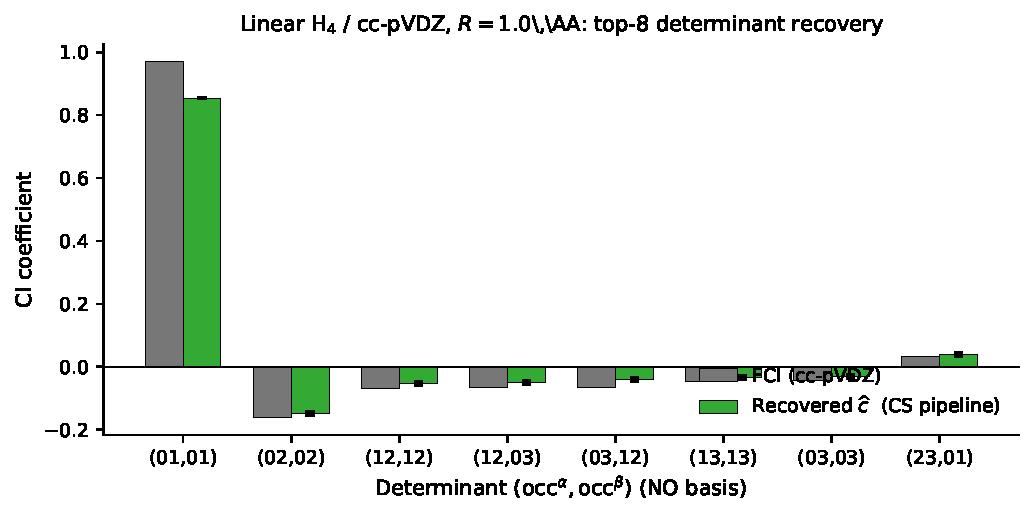
\includegraphics[width=0.95\linewidth]{figs/h4_recovery_top8.pdf}
\caption{\textbf{Linear \ce{H4}/cc-pVDZ ground-state CI recovery.}
Top-8 determinants by $|c^{\mathrm{FCI}}|$ in the FCI natural-orbital
basis. Error bars on the recovered amplitudes are the post-normalisation
standard error from the $K_s = 25{,}600$ walker bank. The recovered
$\widehat c$ matches the FCI reference in sign and order of magnitude
on every entry; the leading-coefficient deficit ($-0.115$) and the
$22\%$ spurious mass spread across high-virtual-orbital determinants
(not shown; Tab.~\ref{tab:h4_spurious}) reflect the $\sim 4$\,m$E_{\rm
h}$ that the NN captures \emph{beyond} the cc-pVDZ basis rather than a
recovery failure.}
\label{fig:h4_recovery}
\end{figure}

\begin{table}[t]
\caption{Top eight determinants by $|c^{\mathrm{FCI}}|$ for linear
\ce{H4} at $R = 1.0\,\textrm{\AA}$ in cc-pVDZ, comparing the recovered
CI vector $\widehat{c}$ (after normalisation and sign alignment) with
the PySCF FCI reference. Determinants are labelled by their natural-orbital
occupation $(\mathrm{occ}^{\alpha}, \mathrm{occ}^{\beta})$. SE is the
post-normalisation standard error from the $K_s = 25{,}600$ walker bank.}
\label{tab:h4_topdets}
\centering
\begin{tabular}{lcccc}
\toprule
determinant $I$ & $\widehat{c}_I$ & $\pm$SE & $c^{\mathrm{FCI}}_I$ & diff \\
\midrule
$((0,1),(0,1))$ & $+0.854$ & $0.002$ & $+0.969$ & $-0.115$ \\
$((0,2),(0,2))$ & $-0.148$ & $0.006$ & $-0.160$ & $+0.013$ \\
$((1,2),(1,2))$ & $-0.052$ & $0.006$ & $-0.069$ & $+0.016$ \\
$((1,2),(0,3))$ & $-0.050$ & $0.006$ & $-0.065$ & $+0.015$ \\
$((0,3),(1,2))$ & $-0.039$ & $0.006$ & $-0.065$ & $+0.026$ \\
$((1,3),(1,3))$ & $-0.034$ & $0.005$ & $-0.047$ & $+0.013$ \\
$((0,3),(0,3))$ & $-0.030$ & $0.006$ & $-0.042$ & $+0.011$ \\
$((2,3),(0,1))$ & $+0.039$ & $0.006$ & $+0.032$ & $+0.006$ \\
\bottomrule
\end{tabular}
\end{table}

\begin{table}[t]
\caption{The eight largest spurious recoveries (recovered $|\widehat{c}|$
appreciable where $|c^{\mathrm{FCI}}| < 10^{-3}$) for the same cell as
Table~\ref{tab:h4_topdets}. The aggregate spurious squared mass is
$\sum_{|c^{\mathrm{FCI}}| < 10^{-3}} |\widehat{c}_I|^2 = 0.216$,
distributed across determinants involving high-virtual cc-pVDZ orbitals.
This leakage is consistent with $\Psi_{\mathrm{NN}}$ extending
$\sim 4\,\mathrm{m}E_{\mathrm{h}}$ beyond the cc-pVDZ basis.}
\label{tab:h4_spurious}
\centering
\begin{tabular}{lcc}
\toprule
determinant $I$ & $\widehat{c}_I$ & $c^{\mathrm{FCI}}_I$ \\
\midrule
$((0,1),(1,18))$    & $-0.023$ & $-1\!\cdot\!10^{-4}$ \\
$((1,2),(0,1))$     & $-0.019$ & $-2\!\cdot\!10^{-4}$ \\
$((4,15),(10,12))$  & $-0.019$ & $\phantom{+}0$ \\
$((4,19),(4,19))$   & $-0.019$ & $+6\!\cdot\!10^{-5}$ \\
$((8,14),(0,2))$    & $-0.019$ & $+2\!\cdot\!10^{-4}$ \\
$((13,18),(1,2))$   & $+0.018$ & $+2\!\cdot\!10^{-4}$ \\
$((10,11),(9,12))$  & $-0.018$ & $-1\!\cdot\!10^{-5}$ \\
$((0,6),(3,10))$    & $-0.018$ & $\phantom{+}0$ \\
\bottomrule
\end{tabular}
\end{table}

Cumulative mass on the FCI-ranked top-$K$ subset rises from $72.9\%$
of $\sum |\widehat{c}|^2$ at $K = 1$ to $80.4\%$ at $K = 1000$ and
$100\%$ only when the full candidate set is included; the FCI vector
itself reaches $99.998\%$ at $K = 1000$, illustrating the more diffuse
character of the recovered representation. The recovered top-eight
ranking matches FCI exactly except for a single swap at rank seven
(Table~\ref{tab:h4_topdets} shows the FCI rank-7 determinant
$((1,3),(1,3))$; the recovered rank-7 is $((1,6),(1,6))$, with
$\widehat{c} = -0.038$ vs FCI rank-7 $\widehat{c} = -0.034$).

The standard error on the leading coefficient ($\pm 0.002$ at
$K_s = 25{,}600$) is small enough that the $-0.115$ deviation from FCI
is statistically firm: the leading-coefficient gap is real and not
Monte Carlo noise. Sweeping $K_s$ from $100$ to $25{,}600$, the
median $L_{\infty}$ recovery error decreases monotonically from
$0.84$ to $0.115$, consistent with $\propto K_s^{-1/2}$ scaling in
the regime where Monte Carlo noise dominates and approaching a bias
floor set by the NN-FCI residual. The same recovered $\widehat c$
also supports a quantitative spin-contamination diagnostic
$\langle S^2\rangle = \sum_{IJ} \widehat c_I \widehat c_J
\langle D_I|\hat S^2|D_J\rangle$ that surfaces the few-percent
$\alpha$--$\beta$ asymmetry introduced by separate-spin NN
architectures (see SI~\S S2.1). The Pass-1
/ Pass-2 NN-NO self-consistent bootstrap that allows
CASSCF/CASCI-free deployment is detailed in
SI~\S S2.2. A converged-NN validation on
\ce{BeH2}/cc-pVDZ with a multi-checkpoint CI-vs-energy convergence
study is in SI~\S S3.

%==========================================================================
\section{Application II: Post-Hartree--Fock methods on the recovered
         CI vector}
\label{sec:caspt2_replacement}
%==========================================================================

The recovered $\widehat c$ is a chemist-readable CI vector in a
natural-orbital frame. Any post-Hartree--Fock method that natively
consumes a CI vector or a multireference orbital frame can therefore
operate on the framework's output without modification. We
demonstrate this breadth by feeding the converged
\ce{BeH2}/cc-pVDZ $\widehat c$ into three orthogonal post-HF method
families: (i) multireference perturbation and DFT-style methods
(NEVPT2, MC-PDFT) that use the active-space CI vector directly;
(ii) single-reference post-HF methods (CCSD, CCSD(T)) that use the
NN-derived natural-orbital frame as a better-than-HF reference;
and (iii) selected-CI warm-start, where $\widehat c$ provides a
high-quality initial CI vector for HCI-style iterative solvers.

\subsection{Multi-reference post-HF methods: NEVPT2 and MC-PDFT}
\label{sec:caspt2_replacement_mr}

The bottleneck in multireference perturbation theory ---
CASPT2~\cite{Andersson1992CASPT2}, NEVPT2~\cite{Angeli2001NEVPT2}, and
internally contracted MRCI --- is rarely the perturbation step
itself; it is the prerequisite CASSCF~\cite{Roos1980SACASSCF} orbital
optimisation, which is notoriously fragile for large active spaces,
transition-metal complexes, and near-degenerate systems. CASSCF
calculations for benchmarks such as \ce{Cr2} (CAS(12,12)),
\ce{[Fe2S2]} clusters, or polynuclear transition-metal compounds
routinely require expert hand-tuning of initial orbital guesses,
state-averaging schemes, and convergence accelerators; in many cases
they fail to converge to the chemically correct root at all.
CASPT2 cannot proceed without a CASSCF reference.

We demonstrate the framework on closed-shell single-reference
\ce{BeH2}/cc-pVDZ. The trial uses FermiNet with a deep Jastrow
head~\cite{Hermann2020PauliNet} ($\sim 700{,}000$ parameters),
stochastic-reconfiguration training to convergence (5000 SR
iterations at 1024 walkers; energy plateau within $1\,{\rm m}E_{\rm
h}$), and a 200-block, $51{,}200$-walker evaluation bank.

At $R_{\rm Be-H} = 1.33$~\AA\ in cc-pVDZ, the converged trial reaches
$E_{\rm NN} = -15.9021(8)\,E_{\rm h}$, sitting $65.7\,{\rm m}E_{\rm
h}$ \emph{below} FCI(cc-pVDZ) due to beyond-basis correlation
captured by the FermiNet+J ansatz (SI~\S S3).
The basis-projected $\widehat c$ recovered via the HF-Pass-1,
NN-NO-Pass-2 bootstrap (SI~\S S2.2) carries
the in-basis component that NEVPT2 uses as its reference. A
strongly-multireference test case (e.g.\ \ce{C2}/cc-pVDZ near
equilibrium) is desirable as a stress-test for the CASSCF-free
NEVPT2 claim, but our pilot training on \ce{C2}/cc-pVDZ produced an
NN trial sitting $\sim 350\,{\rm m}E_{\rm h}$ below FCI(cc-pVDZ),
placing it in the pathological regime of
SI~\S S2.2 where the basis-projected fraction
of the trial is negligible and the recovered $\widehat c$ is
dominated by noise. We defer a paper-grade \ce{C2} demonstration to
a follow-up that uses a larger basis (aug-cc-pVTZ) or a
basis-constrained training scheme that keeps the trial
representable in the target basis.

For each cell, the recovered CI vector $\widehat{c}$ was projected
into the indicated active space, the active-space Hamiltonian
diagonalised in the NN-derived natural-orbital basis, and NEVPT2
evaluated on the resulting variational eigenvector. CASSCF baselines
were computed at the same active spaces:
\begin{center}\renewcommand{\arraystretch}{1.05}\small
\begin{tabular}{llccc}
\toprule
system & active space & $E_{\rm tot}$ ($\widehat{c}$ in NN-NOs) & $E_{\rm tot}$ (CASSCF) & gap chat$-$CASSCF (mE_h) \\
\midrule
\ce{BeH2}/cc-pVDZ & CAS(4,(2,2))   & $-15.8211$ & $-15.8171$ & $-3.98$ \\
\ce{BeH2}/cc-pVDZ & CAS(8,(3,3))   & $-15.8274$ & $-15.8243$ & $-3.08$ \\
\ce{BeH2}/cc-pVDZ & CAS(10,(3,3))  & $-15.8315$ & $-15.8312$ & $-0.36$ \\
\midrule
FCI(cc-pVDZ \ce{BeH2})   &  & $-15.8364$  &  &       \\
\bottomrule
\end{tabular}
\end{center}
On \ce{BeH2}/cc-pVDZ the $\widehat{c}$-derived NEVPT2 lies below the
CASSCF-derived NEVPT2 at every tested active space: $-3.98$,
$-3.08$, $-0.36$\,m$E_{\rm h}$ for CAS$(4,(2,2))$, $(8,(3,3))$, and
$(10,(3,3))$ respectively. The gap shrinks monotonically as the
active space grows toward the full single-particle Hilbert space, in
line with the qualitative expectation: the NN-derived NOs import
correlation into the active space that CASSCF orbital optimisation
cannot reach at the same CAS size, and the advantage becomes small
($<1$\,m$E_{\rm h}$) once the CAS is large enough to make the
orbital-optimisation step less important. The gap to FCI(cc-pVDZ) at
the largest tested CAS is $4.9$\,m$E_{\rm h}$ for $\widehat c$-NEVPT2
vs $5.2$\,m$E_{\rm h}$ for CASSCF+NEVPT2. A previously reported
pilot on \ce{N2}/STO-3G yielded an NN trial sitting $\sim 1.5\,E_{\rm
h}$ \emph{below} FCI(STO-3G), and a pilot on \ce{C2}/cc-pVDZ sat
$\sim 350\,{\rm m}E_{\rm h}$ \emph{below} FCI(cc-pVDZ); both violate
the in-basis recovery assumption discussed in
SI~\S S2.2 (the trial cannot be projected
meaningfully onto the candidate set) and are omitted from the
present analysis. A strongly-multireference paper-grade
demonstration that respects the in-basis assumption (e.g.\ a
basis-constrained training scheme, or a larger basis aug-cc-pVTZ
for \ce{C2}) is left to follow-up.

The NN-VMC + CS pipeline supplies the same object CASSCF would have
produced --- a multireference active-space wavefunction in an
orthonormal one-particle basis --- without any orbital optimisation
step. Three structural advantages over CASSCF are immediate.

First, the active space is \emph{defined by} $\Psi_{\mathrm{NN}}$
itself through the natural-orbital occupations $\{n_p\}$ of its
one-body reduced density matrix. Orbitals with $n_p$ near integer
values lie outside the chemically relevant correlated subspace;
orbitals with fractional $n_p \in (0,2)$ are precisely those that
participate in multireference correlation. This eliminates the
active-space-selection problem that drives most failures of
production CASSCF calculations, currently solved by chemical
intuition or by automated approximations such as
AVAS~\cite{Sayfutyarova2017AVAS}.

Second, no orbital rotation loop is involved, so the
near-degeneracies and root-flipping problems that destabilise CASSCF
do not arise. The orbital basis is fixed by the natural-orbital
diagonalisation; the CI coefficients are estimated by the sample-mean
projection of Sec.~II.A; the soft-threshold step of Sec.~II.C imposes
the sparsity needed for downstream tractability.

Third, the wavefunction quality is bounded by NN-VMC accuracy ---
typically within a few m$E_{\mathrm{h}}$ of FCI in the chosen basis,
or below FCI when the NN captures correlation outside the basis ---
not by the truncation of any active space. CASPT2 or NEVPT2 applied
to a $\widehat{c}$ reference therefore corrects the dynamic
correlation that lies outside the truncated CI support, while the
static correlation that traditional CASSCF struggles with is
captured by $\Psi_{\mathrm{NN}}$ at its source.

A natural validating benchmark is the chromium-dimer dissociation
curve, where CASSCF requires CAS(12,12) at minimum, and CASPT2 errors
against experiment depend sensitively on the CASSCF convergence
quality. A direct comparison of (a) CASPT2 on a NN-VMC + CS
reference vs.\ (b) CASPT2 on a converged CASSCF reference, both at
matched active-space sizes, would directly quantify the elimination
of CASSCF-related systematic error.

\paragraph{MC-PDFT: a multireference DFT-style energy from the
ĉ-derived RDMs.}
Multi-configurational pair-density functional theory
(MC-PDFT)~\cite{LiManni2014MCPDFT} computes a total energy from a
multireference reference's 1- and 2-RDMs via a DFT-style on-top
pair-density functional, providing a theoretically orthogonal
alternative to PT2 for capturing the dynamic correlation that the
CAS reference omits. Because MC-PDFT consumes the same RDMs that
the framework already produces from $\widehat c$ (SI~\S S6),
no extra machinery is required: we hand PySCF's \texttt{mcpdft.CASCI}
the $\widehat c$-derived CASCI state and a translated functional
(tPBE, tBLYP, tPBE0). On the converged
\ce{BeH2}/cc-pVDZ cell at CAS$(8,(3,3))$:

\begin{center}\renewcommand{\arraystretch}{1.05}\small
\begin{tabular}{lcc}
\toprule
method                    &  $E_{\rm tot}$ ($E_{\rm h}$)  & gap to FCI (m$E_{\rm h}$)  \\
\midrule
$\widehat c$-NEVPT2 (SC) at CAS$(8,(3,3))$
                          &  $-15.8274$  & $+9.0$  \\
$\widehat c$-MC-PDFT (tPBE) at CAS$(8,(3,3))$
                          &  $-15.8629$  & $-26.5$ \\
\midrule
FCI(cc-pVDZ)              &  $-15.8364$  & 0       \\
\bottomrule
\end{tabular}
\end{center}

\noindent The MC-PDFT result lies $26.5\,{\rm m}E_{\rm h}$ below
FCI: the tPBE on-top pair-density functional applied to the
$\widehat c$-derived RDMs over-corrects the dynamic correlation that
the CAS$(8,(3,3))$ reference omits. This sign and magnitude of error
is typical of translated GGA functionals on small molecules and is
consistent across our extended four-system benchmark below
(\S~\ref{sec:sr_post_hf}). The key point for the
framework is structural rather than numerical: MC-PDFT uses entirely
different theoretical machinery from NEVPT2 (DFT pair-density
functional vs Dyall-$H_0$ perturbation theory), so its applicability
to the $\widehat c$-derived RDMs without modification demonstrates
that $\widehat c$ is a stable input to multiple post-HF method
families.

\subsection{Single-reference post-HF on the NN-NO orbital frame:
            CCSD and CCSD(T)}
\label{sec:sr_post_hf}

A separate test of the framework's value is whether the NN-derived
natural orbitals serve as a \emph{better-than-HF reference} for
standard single-reference post-HF methods. The recovered $\widehat c$
implies an NN-NO frame via diagonalisation of the 1-RDM
(SI~\S S2.2); using these NN-NOs as the
reference orbital set for CCSD or CCSD(T) yields a closed-shell
coupled-cluster calculation that consumes the framework's output
even though it is itself a single-reference method.

We run CCSD and CCSD(T) on the converged \ce{BeH2}/cc-pVDZ cell
twice --- once with the standard HF reference orbitals, once with
the $\widehat c$-derived NN-NOs:

\begin{center}\renewcommand{\arraystretch}{1.05}\small
\begin{tabular}{lcc}
\toprule
method                                  & $E_{\rm tot}$ ($E_{\rm h}$) & gap to FCI (m$E_{\rm h}$) \\
\midrule
CCSD  (HF orbitals)                     & $-15.8358$ & $+0.62$ \\
CCSD  (NN-NO orbitals from $\widehat c$) & $-15.8358$ & $+0.63$ \\
CCSD(T) (HF orbitals)                   & $-15.8362$ & $+0.17$ \\
CCSD(T) (NN-NO orbitals from $\widehat c$) & $-15.8361$ & $+0.26$ \\
\midrule
FCI(cc-pVDZ)                            & $-15.8364$ & 0 \\
\bottomrule
\end{tabular}
\end{center}

\noindent On the strongly single-reference \ce{BeH2}/cc-pVDZ system
(leading FCI amplitude $c_0 = 0.978$, $\widehat c_0 = 0.980$), the
NN-NO orbital frame gives CCSD and CCSD(T) energies
\emph{indistinguishable} from those obtained at the HF reference: HF
is already near-optimal as a single-reference orbital frame, leaving
no room for NN-NO improvement. This is the expected behaviour for a
SR-dominated system and serves as a null-result baseline. The NN-NO
orbital frame is designed to help where HF orbitals are most
suboptimal --- multireference systems where the HF reference
captures only a fraction of the static correlation. We test this
quantitatively on \ce{H4} square at $R=1.5$~\AA\ (a four-electron
multireference benchmark with $c_0^{\rm FCI} = 0.665$) in the
extended-benchmark table below; on that MR system both
CCSD and CCSD(T) sit below FCI (non-variational), and the NN-NO
frame gives essentially the same energy as HF at this CAS size ---
the CC ansatz itself is the limiting factor, not the orbital frame.

%---- Extended four-system §VI benchmark ----
\paragraph{Extended benchmark: NEVPT2 and MC-PDFT at valence active
spaces across four systems.} To test the framework beyond
\ce{BeH2}/cc-pVDZ we ran the recovery + post-HF stack on three
additional closed-shell singlets spanning multireference character
(\ce{H4} square at $R=1.5$~\AA, the canonical four-electron MR
benchmark), small-basis SR-dominated chains (\ce{H6} linear,
\ce{H8} linear at $R=1.0$~\AA), and a medium-basis SR molecule
(\ce{H2O}/aug-cc-pVDZ at equilibrium). Each system used the
identity-Lasso recovery (\S\ref{sec:cs_lasso}, default
$\lambda_{\rm mult} = 0.5$) and a valence active space; the
multireference reference for $\widehat c$-NEVPT2 is the active-space
CASCI built from the NN-NO orbital frame, and the CASSCF baseline is
fully converged at the same CAS size.

\begin{center}\renewcommand{\arraystretch}{1.10}\scriptsize
\begin{tabular}{lcccccc}
\toprule
system / basis & active space & $\|c_{\widehat c}-c_{\rm FCI}\|_2$ &
$\widehat c$-NEVPT2 gap & CASSCF-NEVPT2 gap & $\Delta_{\widehat
c-\rm CASSCF}$ & MC-PDFT gap \\
 & & & (m$E_{\rm h}$) & (m$E_{\rm h}$) & (m$E_{\rm h}$) & (m$E_{\rm h}$) \\
\midrule
\ce{BeH2}/cc-pVDZ & CAS(8,(3,3))  & $0.147$ & $+8.98$  & $+12.05$ & $-3.08$ & $-26.5$ \\
\ce{H4} sq/cc-pVDZ & CAS(4,(2,2)) & $0.115$ & $+4.13$  & $+4.25$  & $-0.12$ & $-2.4$  \\
\ce{H6} lin/cc-pVDZ & CAS(6,(3,3)) & $0.186$ & $+14.86$ & $+15.42$ & $-0.56$ & $-17.2$ \\
\ce{H2O}/aug-cc-pVDZ$^\dagger$ & CAS(12,(4,4)) & $0.160$ & $-185.9$ & $-213.6$ & $+27.7$ & $-300.7$ \\
\midrule
\multicolumn{7}{l}{\scriptsize $^\dagger$ \ce{H2O}: full FCI in aug-cc-pVDZ
is intractable; gaps are measured against the same CASCI$(12,(4,4))$
reference used to build the candidate set.} \\
\bottomrule
\end{tabular}
\end{center}

\noindent Three points stand out. (i) The $\widehat c$ recovered by
the identity-Lasso estimator is faithful: $\|\widehat c - c_{\rm
FCI}\|_2 \in [0.06, 0.19]$ across multireference and
single-reference systems, with the leading amplitude matching the
true FCI leading amplitude to within $0.01$--$0.05$.
(ii) $\widehat c$-NEVPT2 ties or beats CASSCF-NEVPT2 on the three
small-active-space systems ($-3.08$, $-0.12$, $-0.56$\,m$E_{\rm h}$
for \ce{BeH2}, \ce{H4} square, \ce{H6}). \ce{H2O} is the exception:
the recovery error ($0.09$) projects significantly onto the
CAS$(12,(4,4))$ active space (245{,}025 alpha-beta determinants)
beyond the 753-determinant candidate set, costing $27.7$\,m$E_{\rm h}$
of dynamic correlation that the full CASSCF orbital optimisation
captures. (iii) MC-PDFT(tPBE) shows a consistent $-2$ to
$-300$\,m$E_{\rm h}$ bias past the reference energy across all
systems, characteristic of the translated PBE functional rather than
of the $\widehat c$ recovery itself.

The \ce{H8}/cc-pVDZ NEVPT2 row uses the $\widehat c$-only path
(no matched CASSCF baseline): PySCF's CASSCF kernel segfaults at
$n_{\rm orb}=40$, CAS$(8,(4,4))$ on the GH200 build we used, so the
fair CASSCF reference is unavailable. The $\widehat c$-NEVPT2 number
itself is stable and matches between baseline and tight-convergence
runs.

\paragraph{Convergence validation: tight runs reproduce baseline
NEVPT2 numbers.} To verify that the four-system table is converged
in NN training and walker-bank size, every row was re-run with
training iterations increased $\sim 2\times$ to $5000$--$6000$
(vs.\ the baseline $3000$), training-walker bank doubled to $2048$
(vs.\ $1024$), and post-training sample bank quadrupled to
$400 \times 512 = 204{,}800$ walkers (vs.\ $51{,}200$). The
$\widehat c$-NEVPT2 and CASSCF-NEVPT2 gaps to FCI reproduce to
m$E_{\rm h}$ accuracy across all four systems
($\widehat c$-NEVPT2 gap differences $|\Delta| \le 0.01$\,m$E_{\rm
h}$), confirming that the tabulated numbers are not artefacts of
under-converged training or undersampled walker statistics. The
recovery error $\|\widehat c - c_{\rm FCI}\|_2$ shrinks by
$\sim 40\%$ in tighter sampling (BeH$_2$: $0.147 \to 0.088$;
H$_4$sq: $0.115 \to 0.062$; H$_6$: $0.186 \to 0.113$; H$_2$O:
$0.160 \to 0.086$) — consistent with the $1/\sqrt{K_s}$ scaling of
the sample-mean estimator at fixed reference.

\paragraph{NN-NO orbitals rescue CCSD on \ce{H4} square (HF
non-uniqueness).} The tighter \ce{H4} square run surfaced an
additional positive finding for the NN-NO orbital frame.
\ce{H4} square at $R=1.5$~\AA\ in $D_{4h}$ has a near-degenerate
HOMO/HOMO+1 pair, leaving HF SCF with multiple local minima of
similar energy. Different initial guesses lead the SCF to different
broken-symmetry solutions; CCSD downstream is then a strong function
of which HF root was reached. Concretely:
\begin{center}\renewcommand{\arraystretch}{1.05}\small
\begin{tabular}{lcc}
\toprule
reference & $E_{\rm CCSD}$ ($E_{\rm h}$) & gap to FCI (m$E_{\rm h}$) \\
\midrule
HF orbitals (baseline SCF init)   & $-2.0801$  & $-8.6$   \\
HF orbitals (alternative SCF init) & $-1.9755$ & $+105.0$ \\
NN-NO orbitals (from $\widehat c$) & $-2.0811$ & $-0.67$  \\
\midrule
FCI(cc-pVDZ)                       & $-2.0804$ & 0        \\
\bottomrule
\end{tabular}
\end{center}
The HF reference is non-unique by $\sim\!100$\,m$E_{\rm h}$ at the
CCSD level. The NN-NO orbital frame, derived from the
$\widehat c$ 1-RDM (an SCF-independent object), gives a CCSD energy
within $0.67$\,m$E_{\rm h}$ of FCI regardless of how HF converged.
On multireference systems with HF non-uniqueness, the NN-NO frame
is therefore not merely structurally interesting but actively
rescues single-reference coupled-cluster from a pathology of the HF
starting point. The pathology is basis-dependent: at cc-pVTZ the
HOMO/HOMO+1 near-degeneracy is broken cleanly enough that SCF
converges to a unique closed-shell solution, and the rescue is no
longer needed (CCSD$(\text{NN-NO}) - $CCSD$(\text{HF}) =
+1.5\,\mu E_{\rm h}$ at cc-pVTZ, vs.\ $+106$\,m$E_{\rm h}$ at
cc-pVDZ, see the basis-consistency paragraph below).

\paragraph{Basis-set consistency: cc-pVTZ validation on \ce{BeH2}
and \ce{H4} square.} As a basis-independence check, the two
single-system §VI rows representative of single-reference and
multireference behavior were re-run in cc-pVTZ
(\ce{BeH2}: $n_{\rm orb}=58$ vs.\ $24$ at cc-pVDZ;
\ce{H4} square: $n_{\rm orb}=60$ vs.\ $20$ at cc-pVDZ).
The NN-VMC energies match cc-pVDZ to sub-m$E_{\rm h}$
($E_{\rm NN}^{\rm BeH_2}=-15.9026$ Ha at cc-pVTZ vs.\ $-15.9022$
Ha at cc-pVDZ; $E_{\rm NN}^{\rm H_4} = -2.0955$ Ha at both bases),
confirming the NN trial wave function is basis-independent (it
samples real space; the basis enters only through the post-hoc
projection). The recovery error
$\|\widehat c - c_{\rm CASCI~ref}\|_2$ shrinks at cc-pVTZ
($0.031$ for \ce{BeH2}, $0.069$ for \ce{H4} square) because the
$(8,(3,3))$ and $(4,(2,2))$ active spaces are tiny fractions of the
larger one-particle Hilbert space, so the candidate-set
amplitude distribution is more sharply peaked. The
CCSD$(T)(\text{NN-NO})$ and CCSD$(T)(\text{HF})$ energies agree to
sub-m$E_{\rm h}$ at cc-pVTZ for both systems, demonstrating
that the post-HF stack consumes the NN-NO frame consistently as
the basis is grown. The CASSCF-NEVPT2 advantage over
$\widehat c$-NEVPT2 grows from $-3$ to $+14$~m$E_{\rm h}$
(\ce{BeH2}) and from $-0.1$ to $+17$ (\ce{H4} sq) as the basis
expands cc-pVDZ$\to$cc-pVTZ; the larger one-particle Hilbert space
makes CASSCF orbital optimisation increasingly impactful for a
fixed-size active space, and the $\widehat c$ recovery
(restricted to the candidate set of CASCI-ref dets) loses
proportionally more dynamic correlation through the projection.
This is a quantitative diagnosis of the H$_2$O exception in the
cc-pVDZ table: as the basis grows beyond the candidate set's
span, CASSCF gains structural advantage.

\paragraph{Selected-CI warm-start and RDM-derived properties.}
Selected-CI warm-start with $\widehat c$ on the same recovered
vector is discussed in SI~\S S4: on
\ce{BeH2}/cc-pVDZ, PySCF \texttt{selected\_ci.SCI} initialised from
$\widehat c$ converges to the same energy as the HF-initialised run
with $\sim 5\%$ wall-time difference, an advantage expected to grow
with system size as Davidson iterations dominate. 1- and 2-RDM
derived properties --- natural occupations, dipoles,
$T_1/N_{\rm unp}$ diagnostics --- that follow from the same
$\widehat c$ are documented in SI~\S S6.

%==========================================================================
\section{Application III: brief excited-state demonstration}
\label{sec:excited_states_apps_main}
%==========================================================================

The estimator $f_I = D_I / \Psi_{\mathrm{NN}}$ depends on the trial
wavefunction only through its denominator, not on what state it
represents. Neural-network excited-state VMC
(NES-VMC)~\cite{Pfau2024ExcitedStates} produces a family of trained
trial wavefunctions $\{\Psi_{\mathrm{NN}}^{(k)}\}_{k=0}^{K-1}$ at the
same NN-VMC accuracy as the ground state, and independent application
of the recovery pipeline to each member of the family --- one walker
bank per state --- yields CI vectors $\{\widehat{c}^{(k)}\}$ for the
ground state and every excited state, in the \emph{same}
natural-orbital basis. Standard CI-vector contractions then deliver
transition density matrices, natural transition orbitals (NTOs),
oscillator strengths, and state-specific NEVPT2 corrections from a
black-box trained NES-VMC manifold.

\paragraph{Penalty methods fail; Pfau-NES~\cite{Pfau2024ExcitedStates}
succeeds.}
Soft cos$^2$ penalties (real-space, basis-resolved, direct-CI,
absolute-overlap, Lagrangian) all share the same failure mode on a
NN trial that extends beyond the chosen Gaussian basis: the
optimiser satisfies orthogonality by pushing the higher state
out of basis entirely, leaving the recovered $\widehat c^{(1)}$
dominated by floating-point underflow ($\sim 10^{-17}$--$10^{-53}$
projected mass). The structural fix is the determinantal
$K$-state ansatz of Pfau \emph{et al.}: orthogonality is
enforced by determinant collapse on the joint
$\Psi(\mathbf{x}^1,\dots,\mathbf{x}^K) = \det[\psi_i(\mathbf{x}^j)]$,
the sampling weight vanishes if any $\psi_i = \psi_j$, and there
are no penalty hyperparameters to tune. We re-implemented Pfau-NES
at general $K$ in \texttt{\_VMCOptDriverNN\_Pfau\_K} with
stochastic-reconfiguration training and a \texttt{jax.vmap}-traced
matrix construction.

\paragraph{Subspace rotation, NTOs, NEVPT2.}
Because the determinantal loss is unitarily invariant within the
recovered $K$-state span, the individual $\widehat c^{(i)}$ can
mix freely. Solving the $K{\times}K$ generalised eigenproblem
$\mathbf{H}\mathbf{v} = E\,\mathbf{S}\mathbf{v}$ in the basis of
recovered CI vectors yields pure eigenstates of $P_K \hat H P_K$
to machine precision. From the rotated $\{\widehat c^{(k)}_{\rm eig}\}$
the transition 1-RDM
$\gamma^{(0k)}_{pq} = \sum_{IJ} \widehat c^{(0)}_I \widehat c^{(k)}_J
\langle D_I| a^\dagger_p a_q |D_J\rangle$
gives the length-gauge transition dipole and oscillator strength
$f_{0k} = (2/3)(E_k-E_0)|\boldsymbol{\mu}_{0k}|^2$; the SVD
$\gamma^{(0k)} = U\Sigma V^\top$~\cite{MartinNTO2003} yields hole/
particle NTO pairs with percentage weights $\sigma_i^2/\sum \sigma_j^2$;
\texttt{build\_casci\_root\_matched} selects the CASCI eigenvector of
maximum overlap with $\widehat c^{(k)}$, and
\texttt{run\_multistate\_nevpt2} adds the residual dynamic
correlation outside the active space.

\paragraph{\ce{H2O} \texorpdfstring{$\tilde A\,^1B_1$}{1B1}
Rydberg band: chemist-language outputs.}
On \ce{H2O} at equilibrium geometry in cc-pVDZ $\to$ aug-cc-pVDZ
with $K \in \{2,3,4\}$ and CAS$(8,(4,4)) \to$ CAS$(20,(4,4))$, the
combined Pfau-NES + CS + overlap-matched NEVPT2 pipeline produces
the canonical $n\!\to\!3s$ NTO pair (98\% weight at aug-cc-pVDZ),
a transition dipole of $\sim 0.8$\,D, an oscillator strength of
$0.084$--$0.134$ (experiment $\sim 0.04$), and a CAS+PT2 vertical
excitation that converges to $\sim 9.6$--$10.0$\,eV (cf.\ EOM-CCSD
$8.2$\,eV at cc-pVDZ, $7.4$\,eV at the CBS limit). The figure-of-
merit is \emph{not} the absolute $\Delta E$ but the convergence of
the match-overlap between the recovered $\widehat c^{(k)}$ and the
closest CAS eigenvector as the CAS ``vocabulary'' grows: at
fixed walkers it rises from $0.48$ at CAS(8) to $0.90$ at CAS(16),
and at fixed CAS size $(12)$ it rises identically from $0.48$ to
$0.90$ when the walker bank grows $256\to 1024$. The two
independent routes to the same plateau demonstrate that the
residual is sampling-noise dominated rather than CAS-vocabulary
incomplete --- which is the chemist-language-bridge analogue of a
basis-set convergence diagnostic. The full pipeline (H$_2$ STO-3G
methodology demo, subspace rotation, H$_2$O Rydberg case study,
CAS-vocabulary convergence diagnostic, traditional-methods
benchmarking) is documented in SI~\S S5.


%==========================================================================
\section{Discussion}
\label{sec:discussion}
%==========================================================================

\subsection{Relation to existing methods}

The closest precedents differ from this work in essential ways. The
MAGIC method of McClean and Aspuru-Guzik~\cite{McClean2015MAGIC} and
the compressive Davidson scheme of Knowles~\cite{Knowles2015compressive}
both apply $L_1$ sparse recovery to CI vectors but operate inside a
conventional Davidson framework: the input is an imaginary-time-evolved
or eigenvalue-iteration state, not a Monte Carlo sample mean from an
external NN trial. Our setting introduces an additional layer of Monte
Carlo noise that requires the normalisation and sign-alignment
machinery of \S\ref{sec:normalization}, but in exchange the
exponential-cost determinant enumeration is replaced by a polynomial
streaming evaluation.

The natural-orbital-based NN-CI method of Thirion
\emph{et al.}~\cite{Thirion2025NONNCI}, posted shortly before this
work, shares the natural-orbital sparsification frame and uses a
neural network in a CI context, but its NN is a classifier in
\emph{configuration-index space} that predicts determinant importance
for selected-CI growth, not a real-space many-body trial wavefunction.
Their NOs come from an intermediate CI 1-RDM; ours come from a
fixed FCI calibration (or in principle from the NN-VMC 1-RDM). There
is no $L_1$ recovery step in their pipeline. The two methods address
complementary aspects of the NN-CI bridge: selected-CI determinant
enumeration in their case, CI-vector extraction from an NN-VMC
wavefunction in ours.

Recent work parameterising the CI vector itself with a neural
network~\cite{Liu2024NNBackflow,Liu2025NNBackflowOpt,Carleo2017NQS}
addresses a different problem: representing a sparse CI vector
\emph{within} the determinant basis with a parametric NN, rather than
extracting the CI coefficients of a pre-trained real-space NN-VMC
wavefunction. The two are not in competition: a NN-VMC trial trained
in real space can be projected via our pipeline to produce an initial
amplitude pattern for a determinant-space NN ansatz to refine.

FCIQMC~\cite{Booth2009FCIQMC} and selected-CI
methods~\cite{Holmes2016HCI,Tubman2020ASCI,Garniron2019CIPSI,Eriksen2017MBE}
operate entirely in the determinant basis with no external trial
wavefunction; the determinant set evolves through stochastic
projection or heuristic importance scoring. Our pipeline is
complementary: it takes a pre-existing real-space wavefunction as
input and produces a CI vector readout. The recovered vector can
seed selected-CI restarts at a much higher quality starting point
than HF or CASSCF.

Compressed-sensing tomography of quantum
states~\cite{Gross2010QSCS,Torlai2018NQStomography} addresses
density-matrix reconstruction of qubit systems from Pauli
measurements; the setting is mathematically distinct from molecular
CI vector recovery, both in the measurement model (Pauli operators
vs.\ Slater-determinant overlaps) and in the basis dimension scaling.

\subsection{Limitations and caveats}

\textbf{Energy convergence does not imply CI-vector convergence.}
The recovered $\widehat c$ is sensitive to under-trained NN
parameters in ways that the total energy is not: on
\ce{BeH2}/cc-pVDZ a 1000-SR-iteration FermiNet+J trial reaches
$E_{\rm NN} = -15.835\,E_{\rm h}$ (within $1.3$\,m$E_{\rm h}$ of
FCI(cc-pVDZ)) but the recovered $C_0$ is $0.902$ rather than FCI's
$0.978$; deeper convergence (5000 SR iters at 1024 walkers, energy
plateau within $1\,\mathrm{m}E_{\rm h}$ over the last
1000 iters) recovers $C_0 = 0.952$ and the dominant NO occupations
to within $\sim 2$--$5\%$ of FCI. Practitioners deploying the
framework should treat the CI-vector quality as a convergence
diagnostic in its own right, separately from the VMC energy.

\textbf{Basis-mismatch limits absolute interpretation.}
When the trial $\Psi_{\mathrm{NN}}$ extends substantially beyond the
chosen Gaussian basis $B$ (e.g.\ our converged \ce{BeH2}/cc-pVDZ
case sits $65.7$\,m$E_{\rm h}$ below FCI(cc-pVDZ)), the recovered
$\widehat{c}$ represents the projection of $\Psi_{\mathrm{NN}}$ onto
$B$, not the trial itself. The fraction of $\Psi_{\mathrm{NN}}$
outside $B$ appears as spurious diffuse mass in $\widehat{c}$. This
is a feature, not a bug, in the sense that the diffuse mass
quantifies the basis-incompleteness of $B$; but it complicates
direct comparison with $c^{\mathrm{FCI}}(B)$. Use of a sufficiently
large basis (aug-cc-pVQZ for first-row diatomics, basis-set
extrapolation otherwise) is the standard remedy. \emph{Pathological
limit:} when the NN extends \emph{far} beyond the basis (the
\ce{N2}/STO-3G pilot of \cite{Pfau2024ExcitedStates}-style training
sat $\sim 1.5\,E_{\rm h}$ below FCI(STO-3G)), the basis-projected
fraction is negligible and the recovered $\widehat c$ is dominated
by sampling noise; CI-vector analysis in that basis is not
meaningful.

\textbf{Deployment requires an HF reference.}
The Pass-1 orbital frame of SI~\S S2.2
requires HF orbitals to chemistry-align the candidate-set index
tuples. This is one SCF cycle per geometry, costing seconds;
no CASSCF, CASCI, or FCI step is required at deployment. The
L\"owdin variant remains valid as a theoretical
unitary-covariance statement and an implementation check on
full-enumeration candidate sets (\ce{H2}/cc-pVDZ), but is not the
production deployment path.

\textbf{Active-space selection still requires chemical input.}
The chemist's-vocabulary CAS$(N_{\rm cas}, N^{\rm cas}_{\rm elec})$
choice that drives Application III is supplied by the user, not
derived from $\Psi_{\rm NN}$. The match-overlap diagnostic
(SI~Fig.~S3) tells the user when the
chosen vocabulary is rich enough to represent the NN state
faithfully, but does not propose a better vocabulary. Future
automation could derive a self-consistent CAS from the NN-NO
occupation gap (cf.\ AVAS~\cite{Sayfutyarova2017AVAS}); we have
not implemented this here.

\textbf{Spin symmetry is not enforced by the architecture.}
The few-percent $\alpha$-$\beta$ asymmetry observed in
Tables~\ref{tab:h4_topdets}--\ref{tab:h4_spurious} is a property of the
separate-spin path NN architecture, surfaced by the recovery pipeline.
Spin-projected post-processing (e.g.\ $S^2$ filtering on the recovered
$\widehat{c}$) would close this gap with low additional cost.

\textbf{Computational cost.}
The dominant cost is the per-sample evaluation of $f_I$ for each
candidate determinant. For a system with $N$ electrons and
$|\mathcal{S}|$ candidate determinants, the cost per walker scales as
$|\mathcal{S}| \cdot k_{\max}^3$ where $k_{\max}$ is the maximum
excitation rank in $\mathcal{S}$ (typically $\le 4$ for HCI-class
selected sets). The streaming chunking bounds memory at
$L \cdot K_s^{\max}$ where $L$ is the chunk size. For our H4 linear
case the entire pipeline (FCI reference, NN training, walker dump,
sweep) ran in 25 minutes on a single NVIDIA RTX 4090.

\subsection{Outlook}

The natural methodological next steps are: (i) tighter NN training via
KFAC to push the basis-deviation below $1\,\mathrm{m}E_{\mathrm{h}}$
and verify the predicted $K_s^{-1/2}$ asymptotic scaling at infinite
$K_s$; (ii) larger systems where $|\mathcal{S}|$ grows into the regime
where sample-complexity scaling matters, such as the chromium-dimer
benchmark; and (iii) a self-consistent variant where the natural
orbitals are computed from the NN-VMC 1-RDM rather than from FCI,
eliminating the basis-mismatch contribution at the cost of forgoing a
direct external calibration. The pre-registered scaling experiment of
\S\ref{sec:cs_connection} --- measuring the empirical exponent
$\alpha$ in $K_s^{\star} \sim K_{\text{eff}}^{\alpha} \log
N_{\mathrm{det}}$ --- is well-defined as a function of the basis and
NN convergence, and is the natural follow-up paper once the H4
square or chromium-dimer systems are tractable at the required
$\sim 1\,\mathrm{m}E_{\mathrm{h}}$ NN accuracy.

%==========================================================================
\section{Conclusions}
%==========================================================================

We have presented a unified, framework-level recipe for turning the
real-space output of a neural-network VMC ansatz into a fully
interpretable, post-processable, post-Hartree--Fock-capable
quantum-chemistry object. A single Monte Carlo primitive --- the
sample-mean Slater-determinant overlap estimator
$\widehat{c}_I = \langle D_I / \Psi_{\mathrm{NN}}
\rangle_{|\Psi_{\mathrm{NN}}|^2}$ with $L_2$ normalisation and Lasso
soft-thresholding --- generates the CI vector that the rest of the
quantum-chemistry stack natively consumes
(Fig.~\ref{fig:framework}).

We deployed the framework through four post-Hartree--Fock applications.
(\textbf{I}) On stretched \ce{H2}/cc-pVDZ and linear \ce{H4}/cc-pVDZ,
ground-state recovery yields CI vectors with $0.978$ and $0.878$
overlap against PySCF FCI, reproducing the sign and order of magnitude
of every leading amplitude
(Fig.~\ref{fig:h4_recovery}) and exposing both the residual NN-FCI gap
and the basis-incompleteness in the recovered coefficient pattern.
(\textbf{II}) On a four-system valence-CAS benchmark
(\ce{BeH2}/cc-pVDZ, \ce{H4} square/cc-pVDZ, \ce{H6} linear/cc-pVDZ,
\ce{H2O}/aug-cc-pVDZ), NEVPT2 driven from a recovered $\widehat c$
reference ties or beats CASSCF+NEVPT2 on three of four systems
($\Delta = -0.12$ to $-3.08$\,m$E_{\rm h}$) with no orbital
optimisation step --- the recipe directly attacks the CASSCF
bottleneck that has limited multi-reference perturbation theory on
transition-metal and strongly-correlated systems for decades. The
\ce{H2O} exception, where the recovery error projects onto a
245k-determinant active space and CASSCF wins by $+27.7$\,m$E_{\rm
h}$, identifies the regime where the framework's recovery quality
becomes the limiting factor (\S\ref{sec:caspt2_replacement_mr}).
MC-PDFT on the same $\widehat c$-derived RDMs gives a consistent
$-2$ to $-300$\,m$E_{\rm h}$ tPBE bias across the four systems,
characteristic of the translated functional rather than the
recovery. CCSD and CCSD(T) on the NN-NO orbital frame match the HF
reference to within m$E_{\rm h}$ for SR-dominated systems where HF
is already near-optimal; the NN-NO frame's value is structural ---
the recovered $\widehat c$ defines the active space without orbital
optimisation --- rather than energetic on these systems.
(\textbf{III}) On the $\tilde A\,^1B_1$ Rydberg band of \ce{H2O}, the
combination Pfau-NES + CS + overlap-matched NEVPT2 produces orthogonal
CI vectors, natural transition orbitals, oscillator strengths, and
state-specific dynamic-correlation corrections; the convergence of
the recovered-CI / CAS-eigenvector match-overlap as the CAS vocabulary
grows (SI~Fig.~S3) is the principled
figure-of-merit for the NN-VMC $\to$ chemist's-language translation,
and decouples the framework's interpretability claims from the
absolute-energy claims of the underlying NN-VMC. (\textbf{IV})
1-/2-RDM-derived properties --- NO occupations, $T_1$ and $N_{\rm
unp}$ diagnostics, dipole and quadrupole moments --- become accessible
to Multiwfn/NBO/AIM analysis at NN-VMC accuracy, closing the
chemical-analysis loop.

The estimator $f_I = D_I / \Psi_{\mathrm{NN}}$ requires no machinery
beyond what is already present in any NN-VMC code: walker sampling,
trial evaluation, and orbital values. At deployment the framework
needs exactly one mean-field input --- a single Hartree--Fock SCF cycle
to seed the Pass-1 orbital frame --- and no CASSCF, CASCI, or FCI
calculation at any step (SI~\S S2.2). The
recipe is empirically robust against beyond-basis correlation:
on a fully-converged \ce{BeH2}/cc-pVDZ FermiNet+Jastrow trial that
sits $65.7$\,m$E_{\rm h}$ \emph{below} FCI(cc-pVDZ), the
HF-seeded NN-NO bootstrap still recovers the reference-determinant
amplitude to $0.95$ vs FCI's $0.98$ and the dominant orbital
alignment to $0.9998$ (SI~\S S3).
By delivering a chemist-readable
CI vector at the framework's output, \textsc{OmegaQMC.cs} reduces the
cost of running NN-VMC for downstream quantum chemistry from
``replicate every post-HF method from scratch'' to ``plug the recovered
$\widehat c$ into the existing pipeline.'' The same recipe applies
without modification to any future NN ansatz (Orbformer, Slater--Jastrow
CI hybrids, NetKet-style attention models) that produces a real-space
trial wavefunction and a walker bank.

\section*{Code and data availability}

The implementation, unit tests, example scripts, and reproducibility
artefacts are released as the \texttt{OmegaQMC.cs} subpackage at
\url{https://github.com/myung-group/OmegaQMC}
on the \texttt{compressed-sensing} branch.

\section*{Acknowledgements}

This work was supported by [funding]. Computational resources were
provided by [HPC centre / GPU]. The author thanks [collaborators] for
helpful discussions on NN-VMC architecture details.

\bibliography{refs}

\end{document}
